% Cover letter: Product Manager, dental product portfolio (company not named in the posting)
% CV: Sections/cv_product_manager_dental.tex -> cv_gen/2026-10-27_dental_product_manager/cv_giovanni_tauro-dental_product_manager.pdf
\documentclass[11pt,a4paper,sans]{moderncv}
% Shared preamble and header for the cover letters.
% One main file per application: cl_<company>.tex, built to
% cv_gen/coverletter_giovanni_tauro-<company>.pdf next to cv_giovanni_tauro-<company>.pdf.
% Paths (cl_gen/..., Pictures/...) are relative to the project root, as in the CV (see .latexmkrc).

\moderncvstyle{classic}
\moderncvcolor{blue}

\usepackage[scale=0.80]{geometry}
\setlength{\footskip}{136.00005pt}

\usepackage{fontawesome5}
% hyperref is loaded by moderncv itself; loading it here causes an option clash
\usepackage{xcolor}
\usepackage{graphicx}
\ifxetexorluatex
  \usepackage{fontspec}
  \usepackage{unicode-math}
  \defaultfontfeatures{Ligatures=TeX}
  \setmainfont{Latin Modern Roman}
  \setsansfont{Latin Modern Sans}
  \setmonofont{Latin Modern Mono}
  \setmathfont{Latin Modern Math}
\else
  \usepackage[T1]{fontenc}
  \usepackage{lmodern}
\fi

\usepackage[english]{babel}

% used for the PDF title and the letter closing; the visible header is \clheader below
\name{Giovanni}{Tauro}

% Header: #1 = headline under the name (same as the headline of the matching CV)
\newcommand{\clheader}[1]{%
\noindent
\begin{minipage}[c]{0.74\textwidth}
    {\Huge \textbf{Giovanni Tauro}}\\[-0.2em]
    {\small #1}\\[0.3em]

    \footnotesize
    \faMapMarker*~
    \href{https://www.google.com/maps/search/?api=1&query=Lecco+23900+Italy}
    {\color{blue}Bari-Lecco, Italy}
    \quad
    \faPhone*~
    \href{https://wa.me/393279437161}
    {\color{blue}+39 3279437161}
    \quad
    \faEnvelope~
    \href{mailto:giovanni.taurodi@gmail.com}
    {\color{blue}giovanni.taurodi@gmail.com}
    \\[-0.1em]

    \faLinkedin~
    \href{https://www.linkedin.com/in/giovanni-tauro-gt/}
    {\color{blue}LinkedIn}
    \quad
    \faGithub~
    \href{https://github.com/jotades}
    {\color{blue}GitHub}
    \quad
    \faGraduationCap~
    \href{https://scholar.google.com/citations?user=BS0aVGgAAAAJ&hl=it}
    {\color{blue}Scholar}
    \quad
    \faFilePdf~
    \href{https://www.notion.so/Giovanni-Tauro-2a7901d92f3a800b892af425c5875c6a}
    {\color{blue}Portfolio}
    \quad
    \faCubes~
    \href{https://grabcad.com/giovanni.tauro-3}
    {\color{blue}GrabCAD}

\end{minipage}
\hfill
\begin{minipage}[c]{0.18\textwidth}
    \raggedleft
    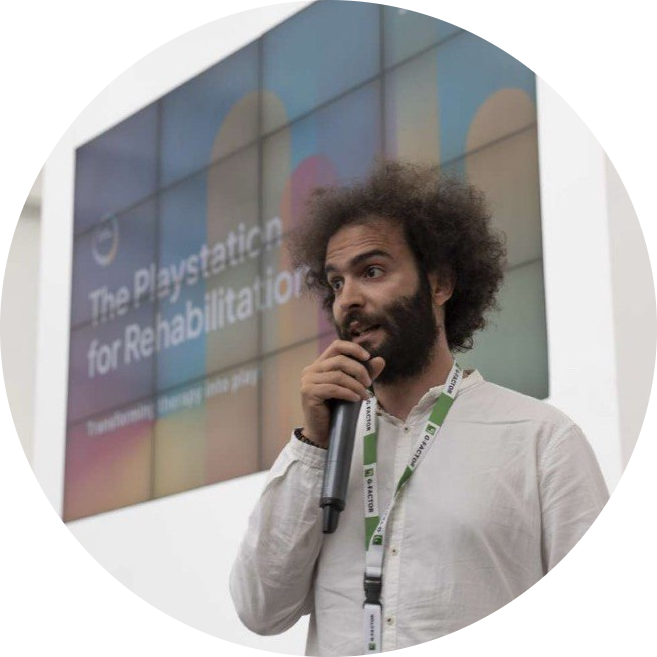
\includegraphics[width=2.8cm]{Pictures/Giovanni_pitch}
\end{minipage}
\vspace{0.1em}
}

\makeatletter
% the sender details are already in \clheader, so skip moderncv's own block
\@detailsfalse
% closing phrase, signature, name
\renewcommand*{\makeletterclosing}{%
  \@closing\\[0.6em]%
  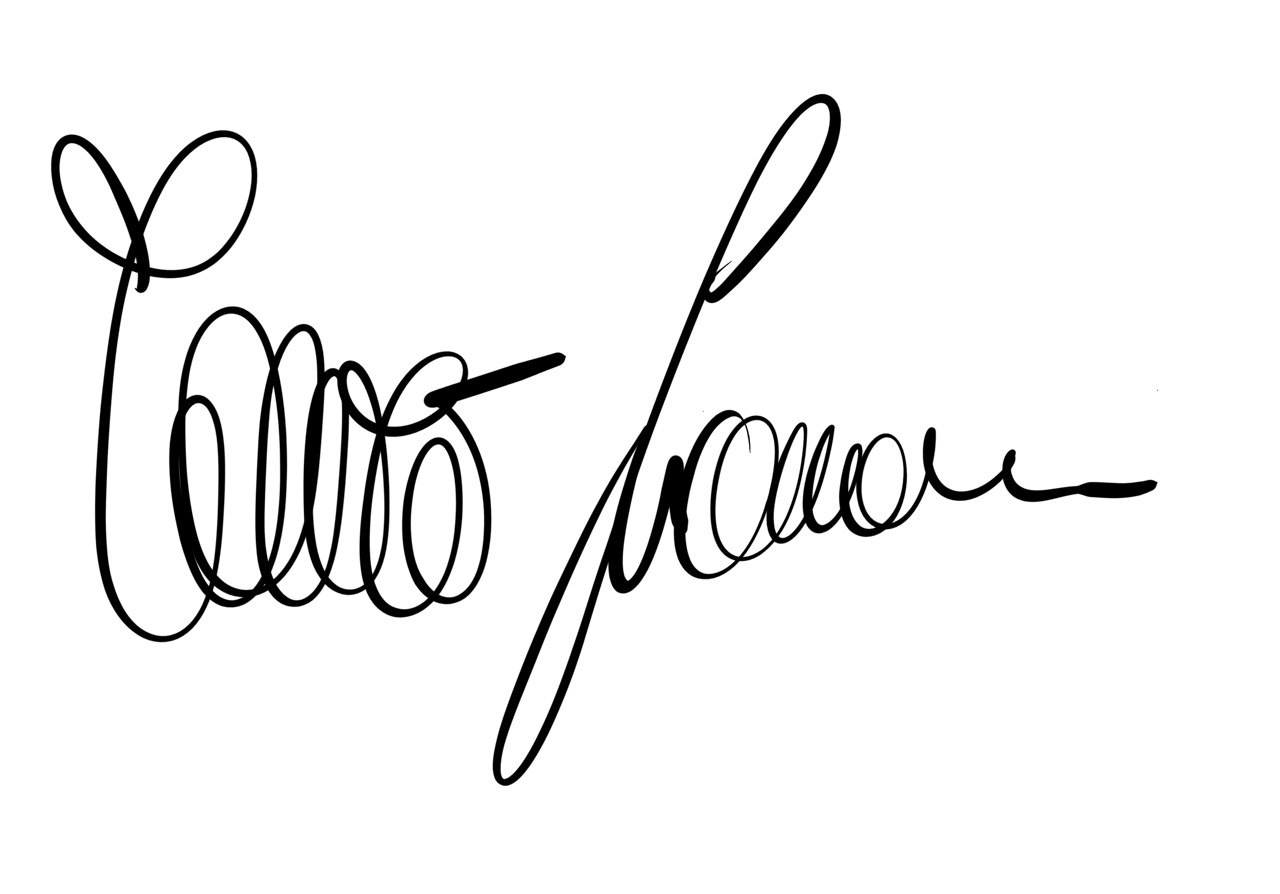
\includegraphics[height=1.2cm]{Pictures/sign_gt.jpg}\\[0.2em]%
  {\bfseries\@firstname~\@lastname}}
\makeatother


\begin{document}

\clheader{Head of Product | Regulated Medical Devices}

\recipient{Hiring Team}{Product Manager, Dental}
\opening{Dear Hiring Team,}
\closing{Sincerely,}
\makelettertitle

I am applying for the Product Manager role for your dental product line. I am Head of Product and co-founder of Rehabilia Technologies, and for more than five years I have developed medical devices at CNR-STIIMA, the Italian National Research Council.

Dentistry is where my product work began. For my MSc thesis at Politecnico di Milano I designed WashB, an ultrasonic teeth-cleaning device. I started from research on brushing, flossing, materials and people's oral-care habits, which pointed to ultrasound as a way to remove biofilm in areas that brushing and flossing miss. The device had to work regardless of the user's manual dexterity and adapt to different dental arch shapes, and I chose its materials and optimised the shape of its functional components.

Since then I have taken a regulated device from concept to clinic. PhiCube, a rehabilitation device of which I am co-inventor (WO2023214349A1), went from interviews with clinicians and hardware/software requirements to deployment in Italian clinics, under MDR, ISO 13485 and IEC 60601. I contributed to its CE-oriented technical files, manuals and design dossiers, turning regulatory requirements into design inputs. PhiCube reached a usability score of 85.8/100 (SUS) with 19 children and is now in two ongoing multicentre studies with 134 patients.

As Head of Product I run field research with clinics on their pain points, the tools they use and how they make purchasing decisions, and turn it into requirements, a prioritised backlog and a milestone-based roadmap. I align engineers, clinicians, research partners and suppliers on scope, timelines and trade-offs, and I base decisions on usability tests and study data. In the EIT Health MedTech and EIT Wildcards bootcamps I worked on our business and financial plan, and I regularly present the product to clinicians, partners and support programmes.

My regulatory experience is with the EU MDR rather than the FDA, and I have not yet launched a product through a sales organisation or worked with distributors and DSOs. These are the areas where I would expect to learn the most in my first months. I am used to 3D scanning and CAD workflows from my earlier work, which should help with digital dentistry, and I am happy to travel.

I would welcome the chance to discuss the role further.

\makeletterclosing

\end{document}
